\documentclass[11pt]{article}
\usepackage{mypackages}
\begin{document}

\section{Results}

For each of the experiments described in the previous section, we will be using
\textit{timesteps} as a time unit.
The time step is increased every time an action is performed and a new state is encountered.
Thus it describes the amount of state transitions performed, and in order to make the setting
fair for all the thread settings, the training was done such that all of the settings
made the same amount of transitions.

\subsection{Playing CartPole - Actor-Critic with eligibility traces}

For this experiment our implementation was allowed to take at most 200.000 timesteps.
The pace of learning depends on the “luck” of the exploration.
Therefore we ran the experiment five times to only show the average performance of
the algorithm.
In figure \ref{fig:cp_et} the results of the experiment is shown
as a function of real-time and timesteps.
Since this method is using only a single thread the two plots should show the same.
% Template
\begin{figure}[H]
    \begin{tabular}[c]{c}
    \begin{subfigure}{\textwidth}
        \centering
        \fbox{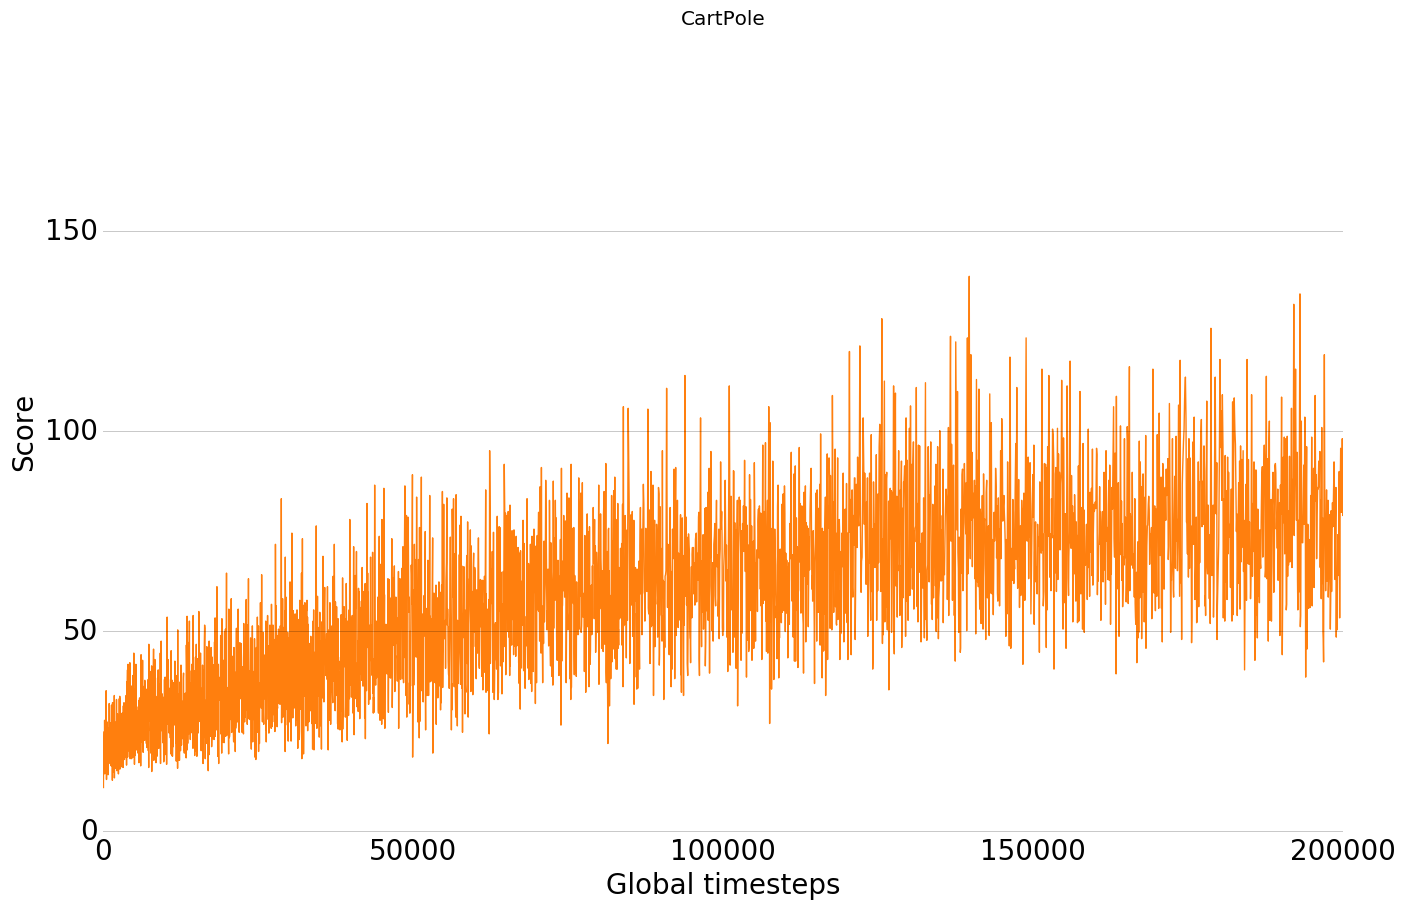
\includegraphics[scale=0.4]{plots/eligibility_steps.png}}
        \caption{The score of the Actor-Critic method with eligibility
            traces as a function of the number of timesteps
            the algorithm have been running.}
    \end{subfigure}
    \end{tabular}
    \begin{tabular}[c]{c}
    \begin{subfigure}{\textwidth}
        \centering
        \fbox{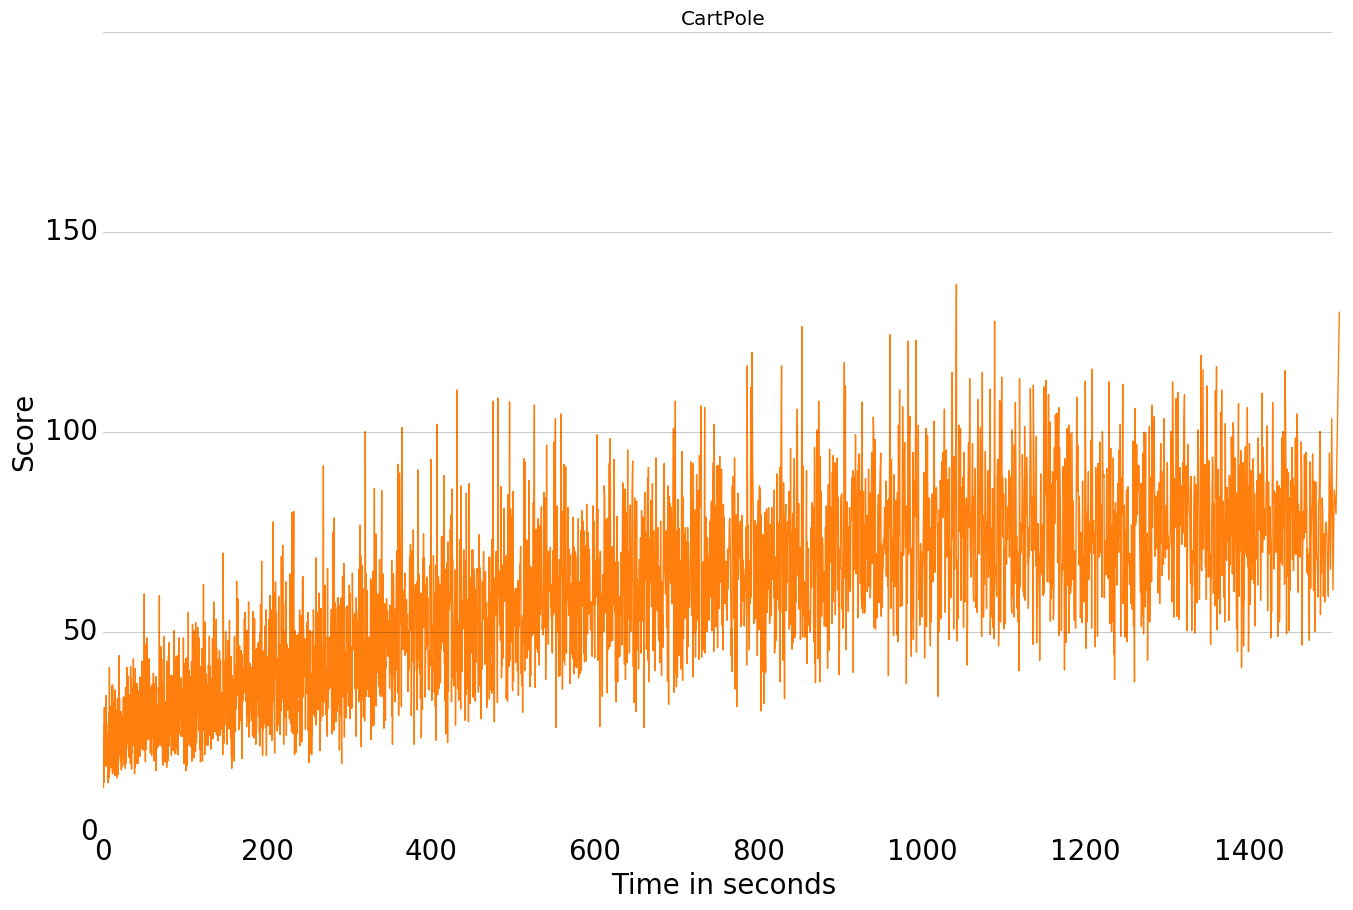
\includegraphics[scale=0.415]{plots/eligibility_time.png}}
        \caption{The score of the Actor-Critic method with eligibility
            traces as a function of the real-time the algorithm
            have been running.}
    \end{subfigure}
    \end{tabular}
    \caption{Average results of five runs of the Actor-Critic method
    with eligibility traces.} 
     \label{fig:cp_et}
\end{figure}

Unlike the Atari games, CartPole can be won if the player reaches a score of 200.
The results of our experiments suggest that
the method isn't able to learn to solve the game completely,
since the highest mean score is 138.8, which is achieved after 139.688 timesteps.
However, that it was able to achieve this score shows
that it learned a decent policy - just not the optimal one.
This result reinforces the hypothesis that the implementation of the
Actor-Critic method with eligibility traces is suboptimal, even
though the average mean increased over the course of the experiment.
It is notable that the method is stable in the sense that once it has found
a policy, it won't learn a policy that produces a worse result.


\subsection{Playing CartPole - A3C}

In this experiment we also allowed the implementation to run for
200.000 timesteps.
Again the experiment was run five times to avoid “lucky”, and “unlucky”, runs
interferring with the result. 
Figure \ref{fig:a3c_time_steps} and \ref{fig:a3c_time} shows the average result of the experiments for all thread settings - that is 16 threads, 8 threads, 4 threads,
2 threads and 1 thread.
Due to the natural variance in the results, as is prominent in figure \ref{fig:cp_et},
we have smoothed the results such that each point represent the mean of the 50
surrounding points.
We have applied the smoothing to make the plots more readable and
thus they should only be interpreted as the “trend” of the
result.

\begin{figure}[H]
    \centering
    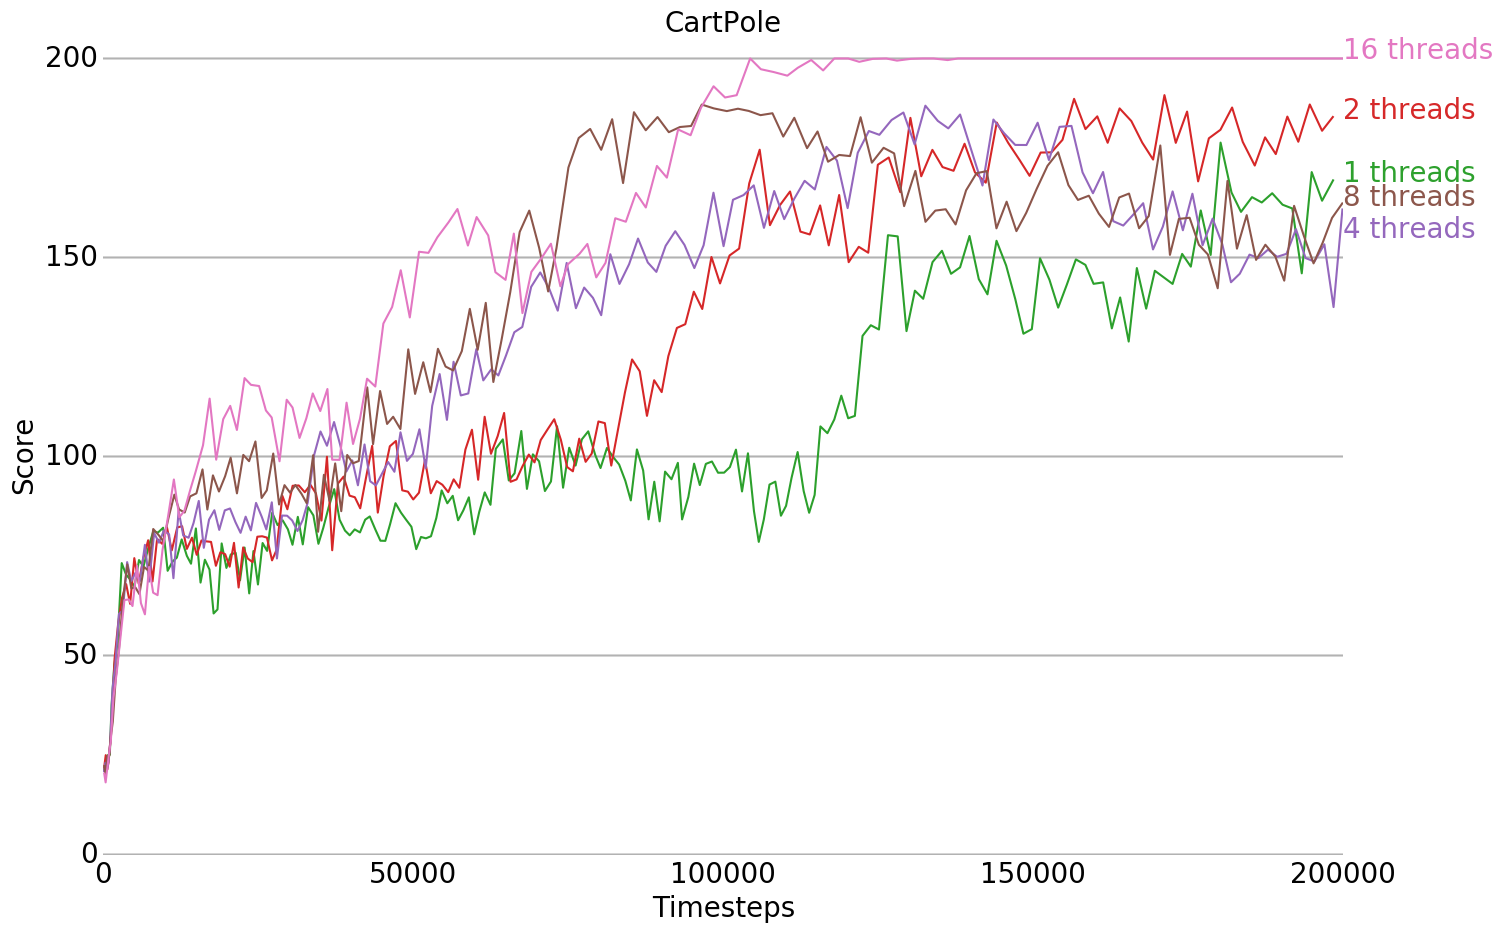
\includegraphics[scale=0.4]{plots/cartpole_compare_counter_without_AC.png}
    \caption{The score of the A3C method in CartPole as a function
    of the number of timesteps the algorithm have been running.}
    \label{fig:a3c_time_steps}
\end{figure}
 

When looking at figure \ref{fig:a3c_time_steps}, we how the
performance increases over time, as we learn a optimal policy. 
Most of the learning seems to happen in the first 120.000 timesteps,
hereafter the gradient of the performance become smaller, which
meas that we don't get siginifacant improvement from this point.
For all the different amounts of threads used it the implementation
is converging towards a constant mean score of 200 and even reaches
it for 16 threads.
It seems like the implementation is stable for all thread settings, with a slight
drop in performance after roughly half the timesteps using 8 threads.
This result was not unexpected, as the same amount of timesteps should produce similar
scores for this relatively simple problem. 

\begin{figure}[H]
    \centering
    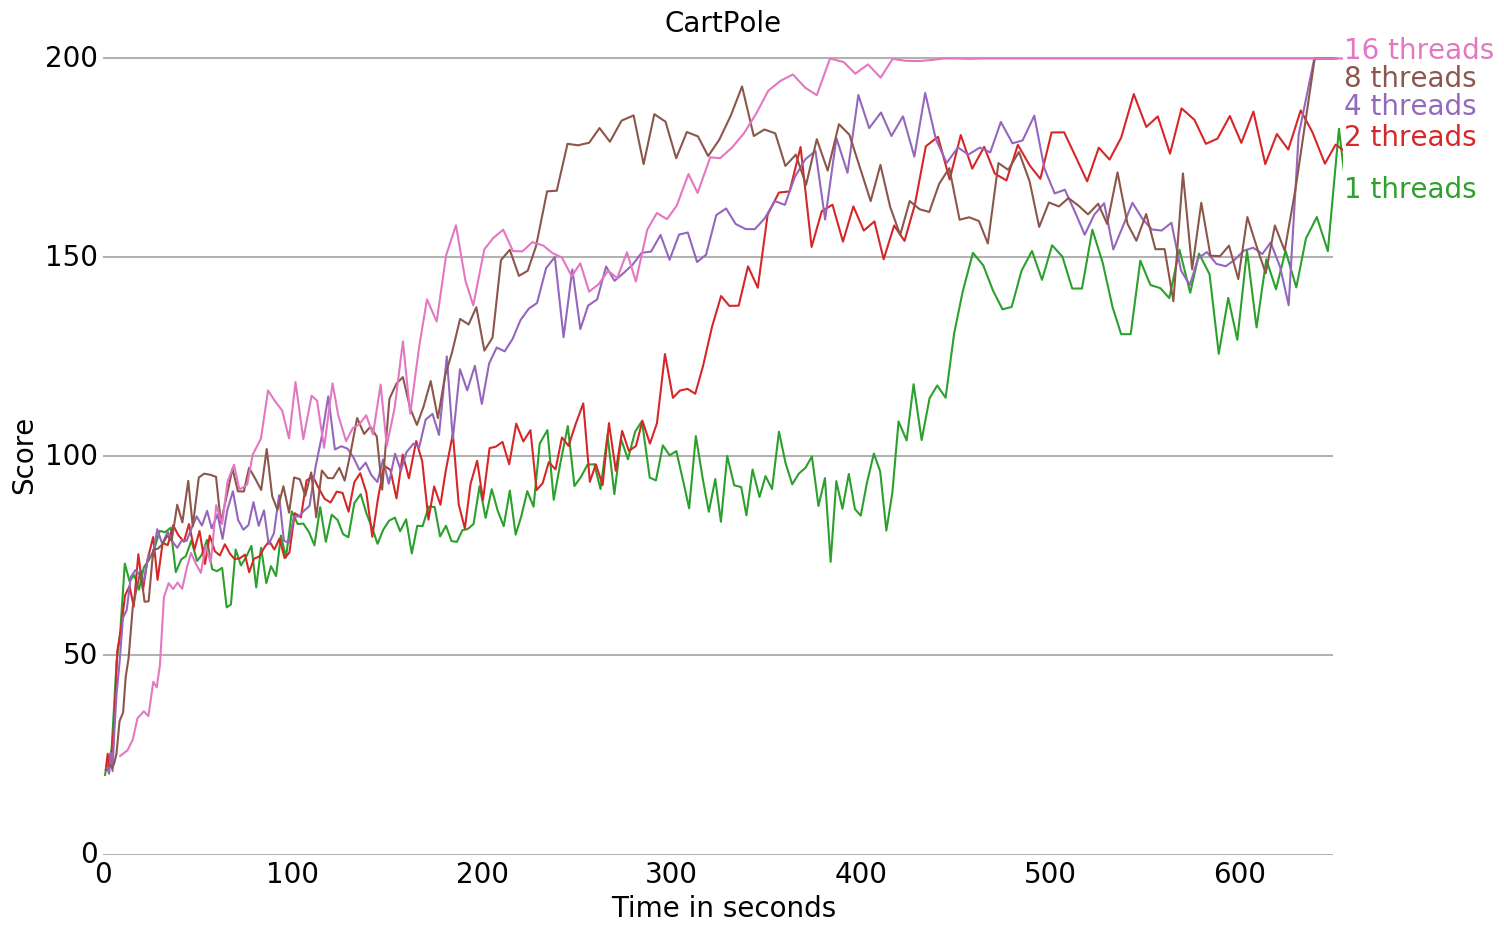
\includegraphics[scale=0.4]{plots/cartpole_compare_time_without_AC.png}
    \caption{The score of the A3C method in CartPole as a function
    of the amount of real-time the algorithm have been running.
    Here the plot has been cut off after the first thread setting
    terminated.}
    \label{fig:a3c_time}
\end{figure}

It is notable that the plots of real-time and timesteps are almost identical, which
is surprising since the usage of more threads didn't achieve a significant speedup
in real-time used by the implementation.


%\begin{figure}[H]
%    \begin{tabular}[c]{c}
%    \begin{subfigure}{\textwidth}
%        \centering
%        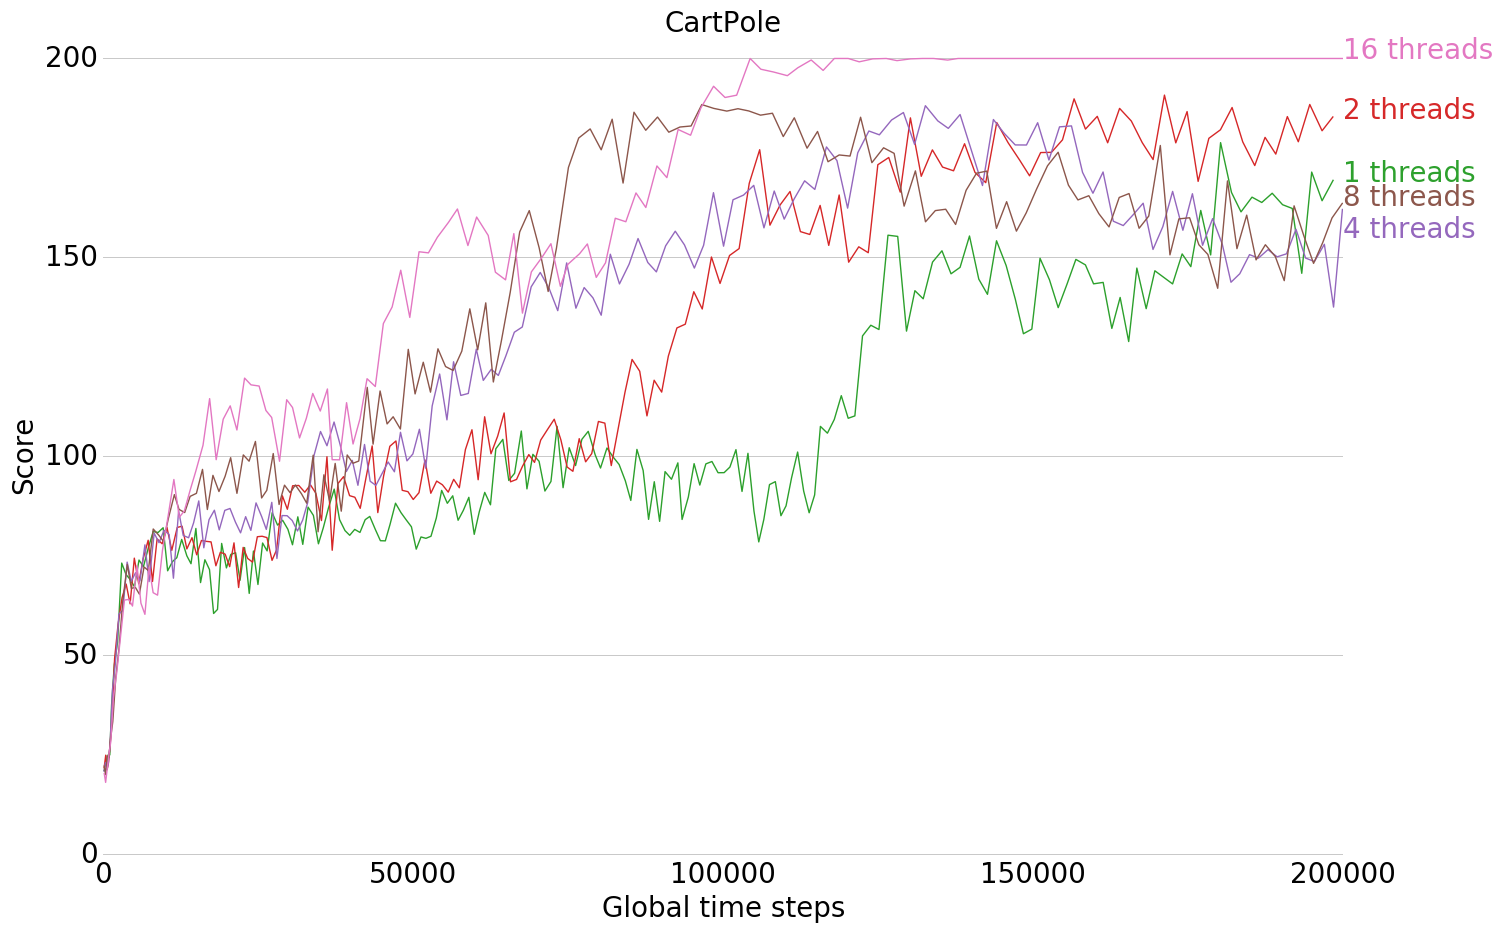
\includegraphics[scale=0.4]{plots/cartpole_compare_k50_steps.png}
%        \caption{The score of the A3C method in CartPole as a function
%        of the number of timesteps the algorithm have been running.}
%    \end{subfigure}
%    \end{tabular}
%    \begin{tabular}[c]{c}
%    \begin{subfigure}{\textwidth}
%        \centering
%        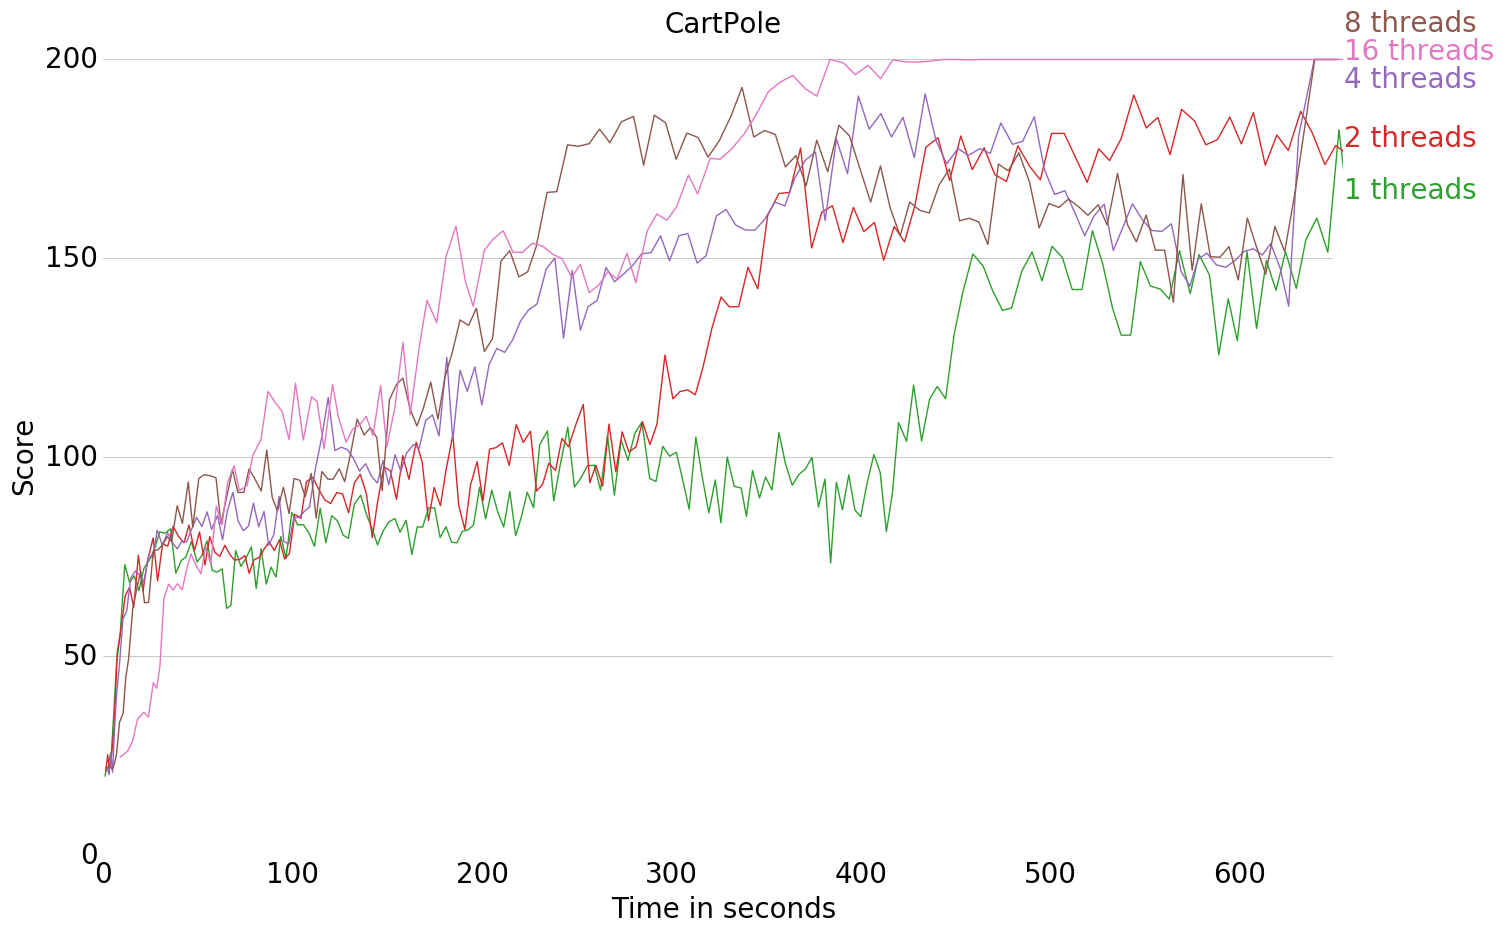
\includegraphics[scale=0.4]{plots/cartpole_compare_k50_time.png}
%        \caption{The score of the A3C method in CartPole as a function
%        of the amount of real-time the algorithm have been running.}
%    \end{subfigure}
%    \end{tabular}
%    \caption{Average results of the A3C implementation playing the CartPole
%        game. The plots describe the mean of the surrounding 50 points.}
%     \label{fig:a3c_cp_all}
%\end{figure}


\subsubsection{Comparison between different amounts of threads}

Figure \ref{fig:a3c_comp_steps} shows the average result obtained from running 200.000
timesteps five times for each thread setting.

\begin{figure}[H]
  \centering   
  \begin{tabular}[c]{cc}
    \begin{subfigure}[c]{.5\textwidth}
        \fbox{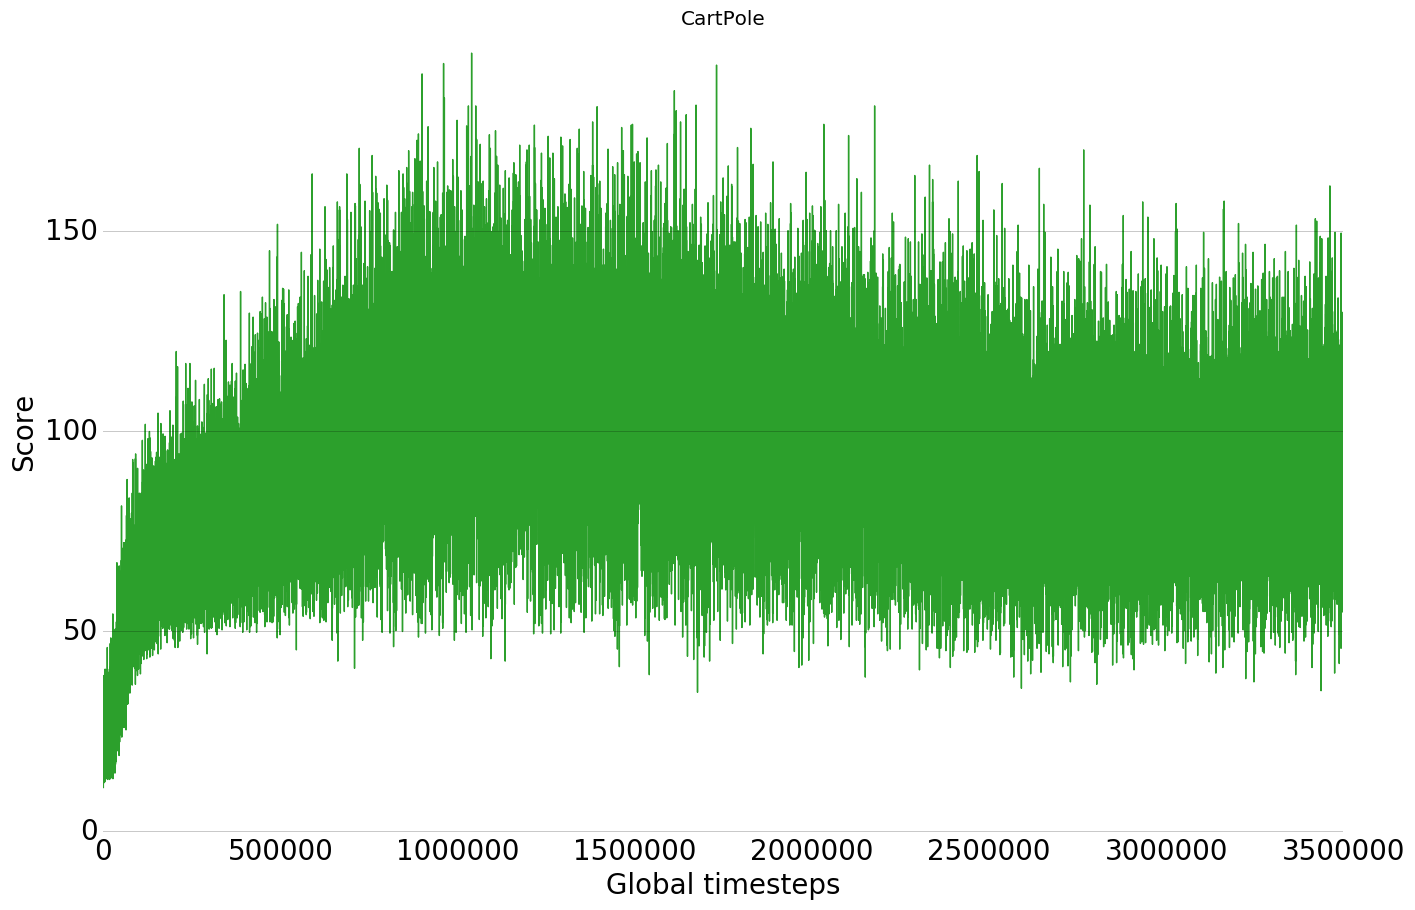
\includegraphics[width=0.95\textwidth]{plots/cartpole_1_threads.png}}
        \caption{A3C playing CartPole using 1 thread.}
        \label{cp:1}
    \end{subfigure}
    \begin{subfigure}[c]{.5\textwidth}
        \fbox{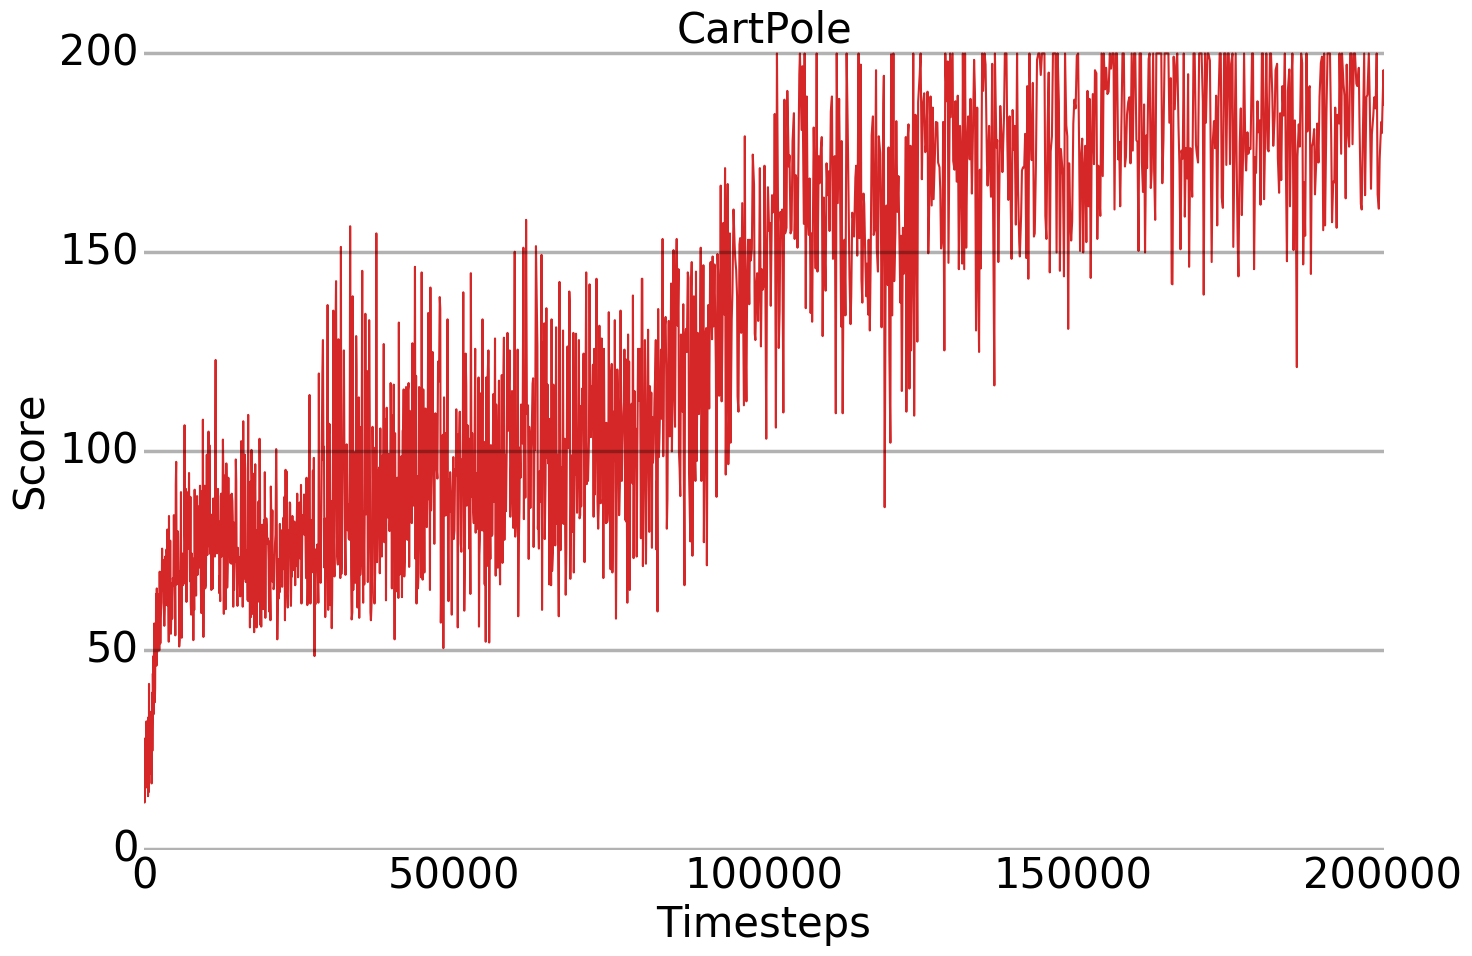
\includegraphics[width=0.95\textwidth]{plots/cartpole_2_threads.png}}
        \caption{A3C playing CartPole using 2 thread.}
        \label{cp:2}
    \end{subfigure}
  \end{tabular}
  \begin{tabular}[c]{cc}
    \begin{subfigure}[c]{.5\textwidth}
        \fbox{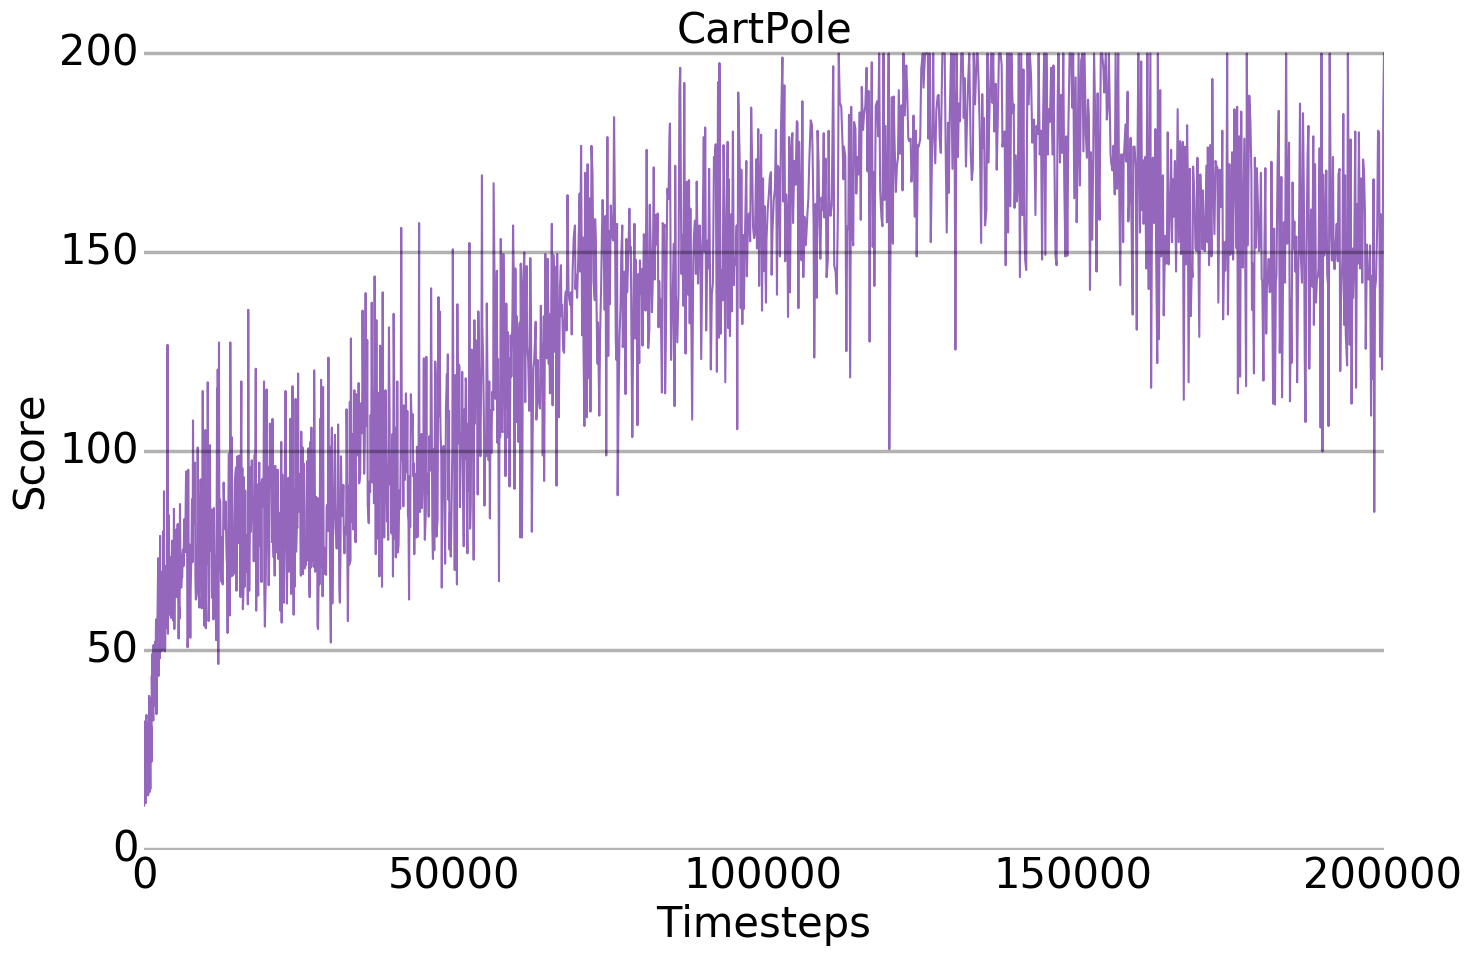
\includegraphics[width=0.95\textwidth]{plots/cartpole_4_threads.png}}
        \caption{A3C playing CartPole using 4 thread.}
        \label{cp:4}
    \end{subfigure}
    \begin{subfigure}[c]{.5\textwidth}
        \fbox{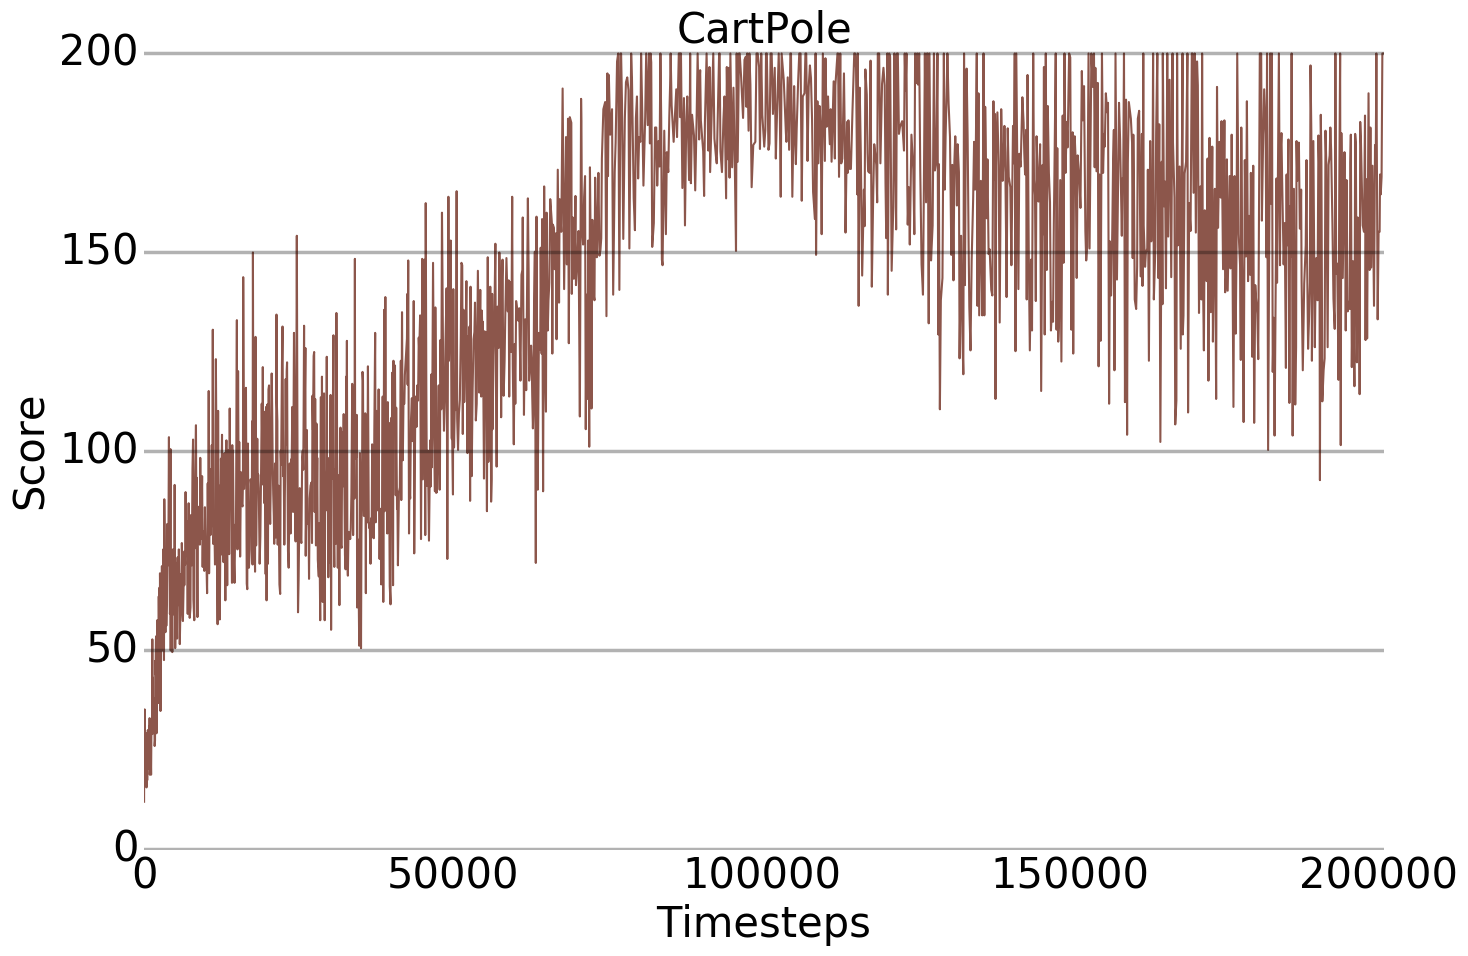
\includegraphics[width=0.95\textwidth]{plots/cartpole_8_threads.png}}
        \caption{A3C playing CartPole using 8 thread.}
        \label{cp:8}
    \end{subfigure}
  \end{tabular}
  \begin{tabular}[c]{c}
    \begin{subfigure}[c]{.5\textwidth}
        \fbox{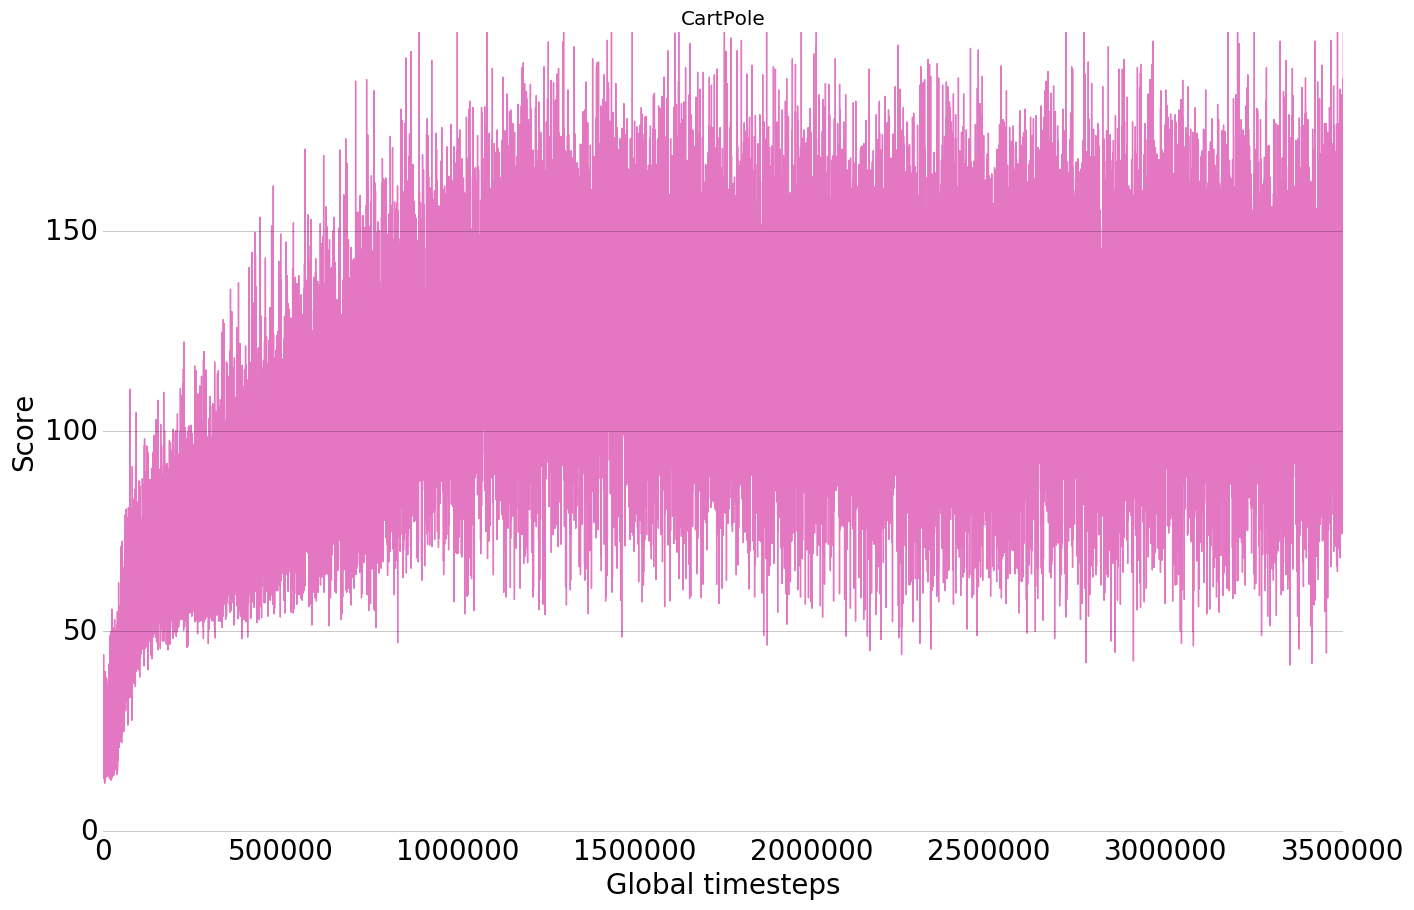
\includegraphics[width=0.95\textwidth]{plots/cartpole_16_threads.png}}
        \caption{A3C playing CartPole using 16 thread.}
        \label{cp:16}
    \end{subfigure}
  \end{tabular}
  \caption{The scores of all the different thread settings for the
    A3C implementation playing CartPole as a function of timesteps taken.}
     \label{fig:a3c_comp_steps}
\end{figure}

Again it seems as if the scores converge at roughly the same pace,
upon further inspectation of the results.
It is notable that the variance of in scores is also approximately
the same for all thread settings, but only the experiment using 16 threads
can keep a stable mean score of 200.


\subsubsection{Comparison between A3C and Actor-Critic method using eligibility traces}

Figure \ref{fig:a3c_comp_eligibility} shows a comparison between the
results of the A3C algorithm and the Actor-Critic method with eligibility
traces.
The plots have been smoothed such that each point is the mean of the surrounding 50,
to increase the readability of the comparison.
Again the plots only show the trend of the results, but it will be sufficient
for our aim.

\begin{figure}[H]
    \centering
    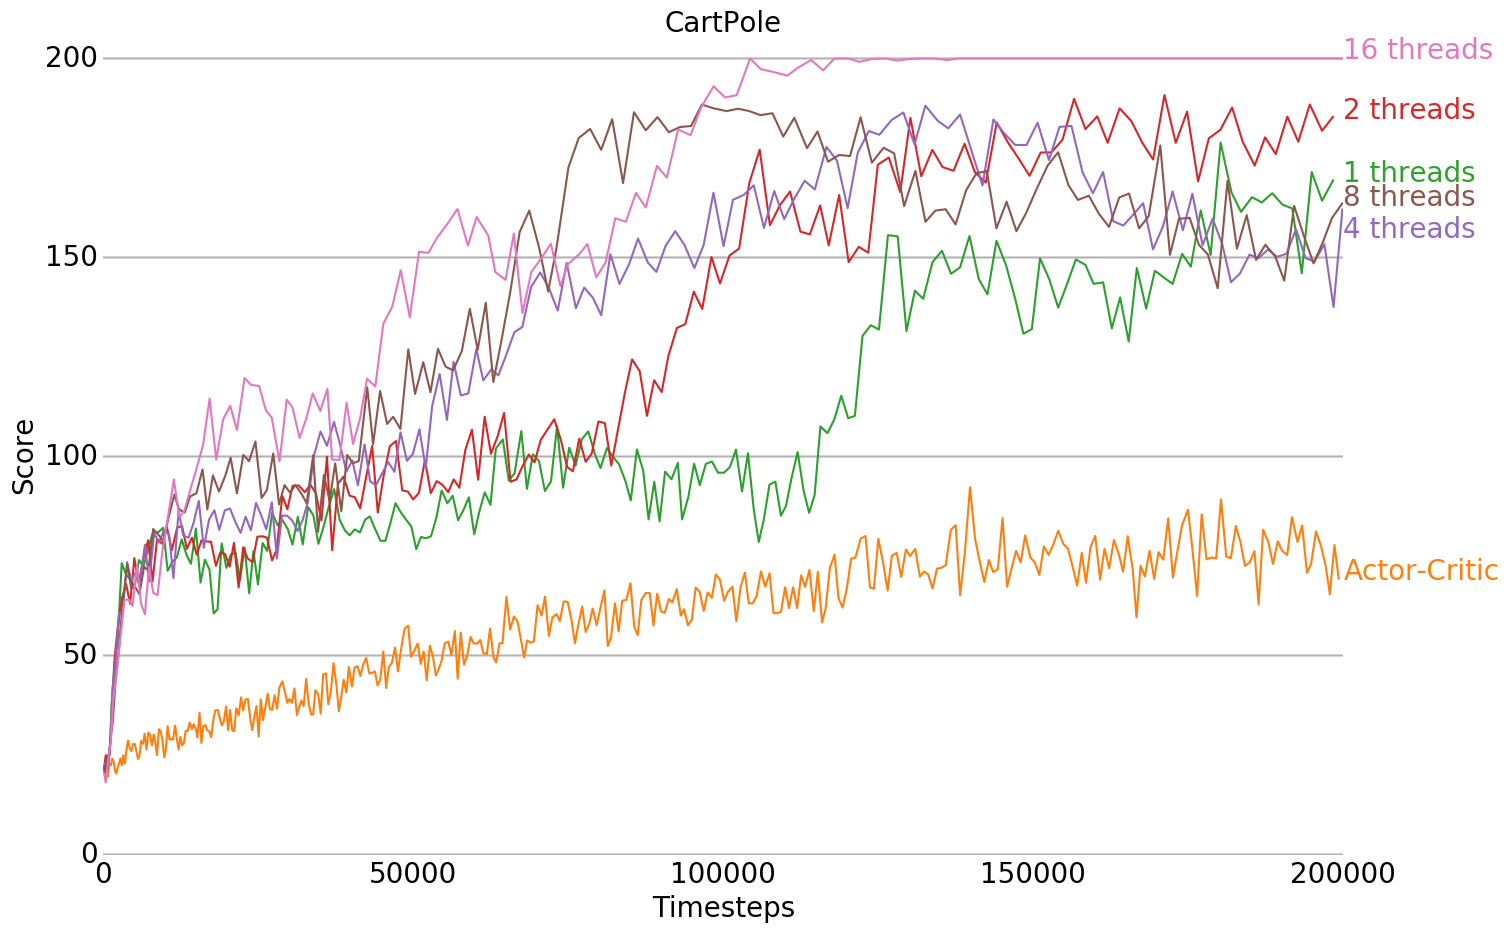
\includegraphics[scale=0.4]{plots/cartpole_compare_counter_with_AC.png}
    \caption{The results of the A3C algorithms different thread
            settings compared to the result of the Actor-Critic method
            with eligibility traces.}
    \label{fig:a3c_comp_eligibility}
\end{figure}

From the comparison it is easy to see that the A3C algorithm is performing
better in regards to pace of learning and overall final mean.
However, the Actor-Critic with eligibity traces seem to present less variance
in its mean scores and learning curve.

\subsection{Playing Atari games}

In CartPole we allowed our implementation to run for 200.000 timesteps.
However, due to the immense computational time required to
learn to solve the problem we have instead defined the limit of the
Atari implementation as 16 hours worth of training time.

Figure \ref{fig:all_atari} shows the average score over the amount of
experiments that were performed for each of the games we tested.
To show the trend of the A3C we smooth the plots such that
each point represents the mean of the 500 surrounding points.

\begin{figure}[H]
  \begin{tabular}[c]{ccc}
    \begin{subfigure}[t]{.33\textwidth}
        \fbox{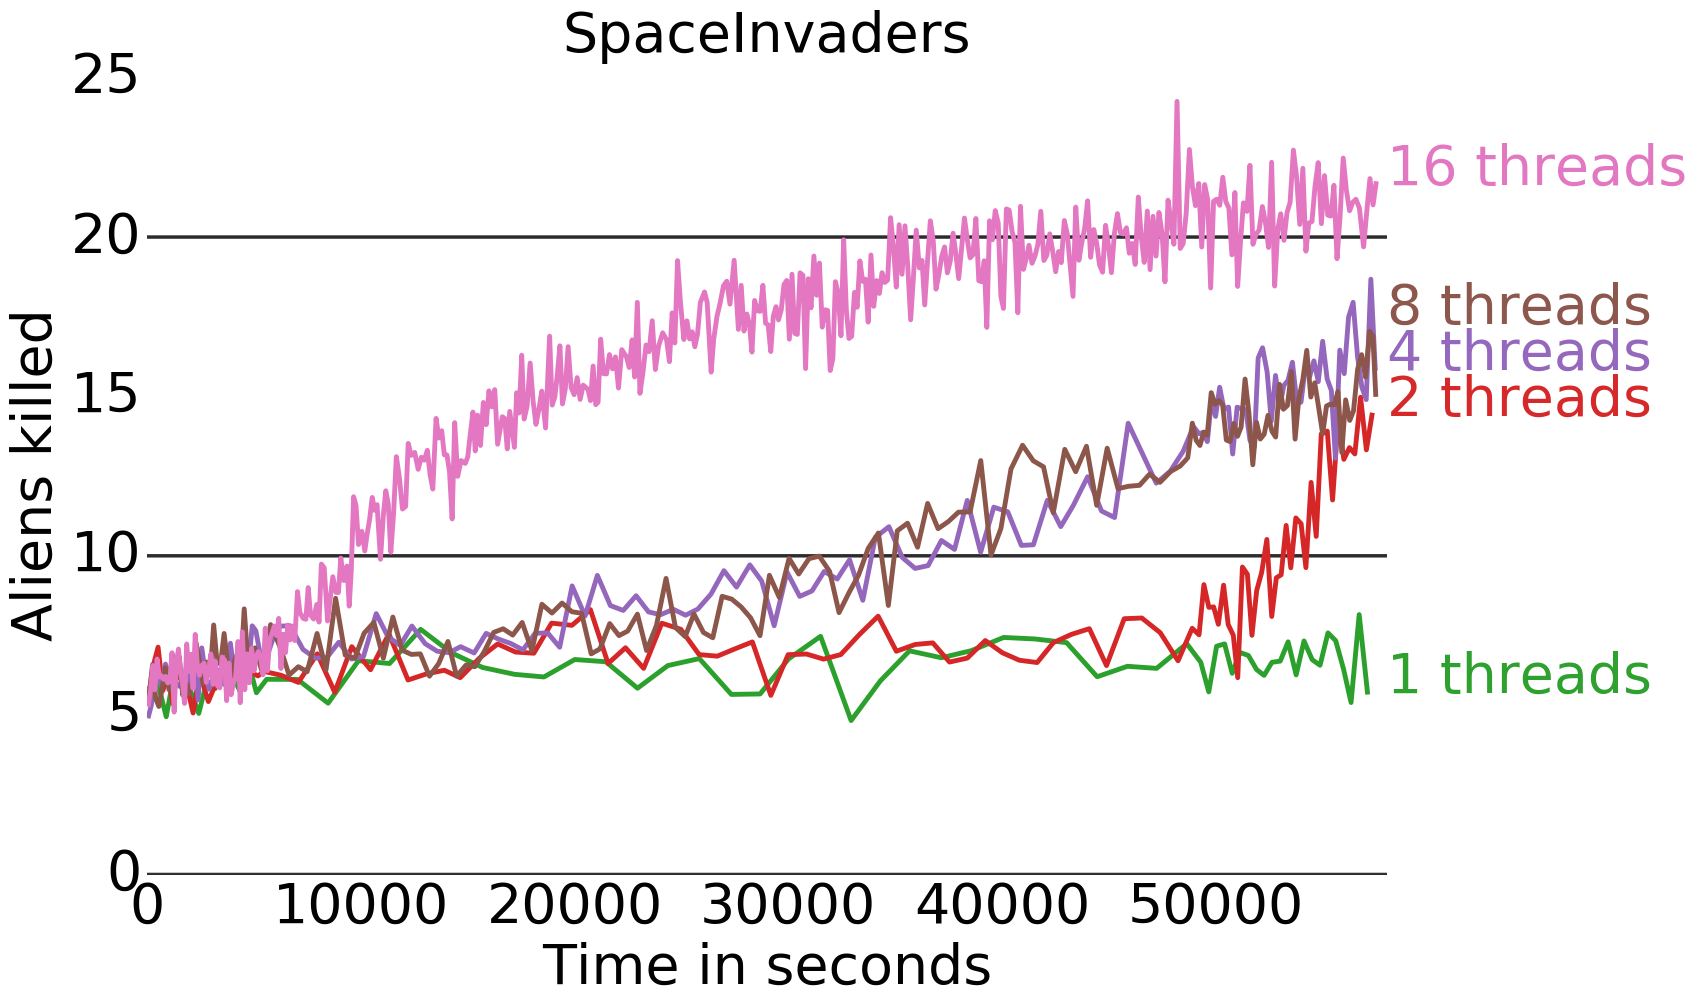
\includegraphics[width=.95\textwidth]{plots/spaceinvaders_intro.png}}
        \caption{Score achieved in Space Invaders as a function of
        consumed real-time.}
    \end{subfigure}
    \begin{subfigure}[t]{.33\textwidth}
        \fbox{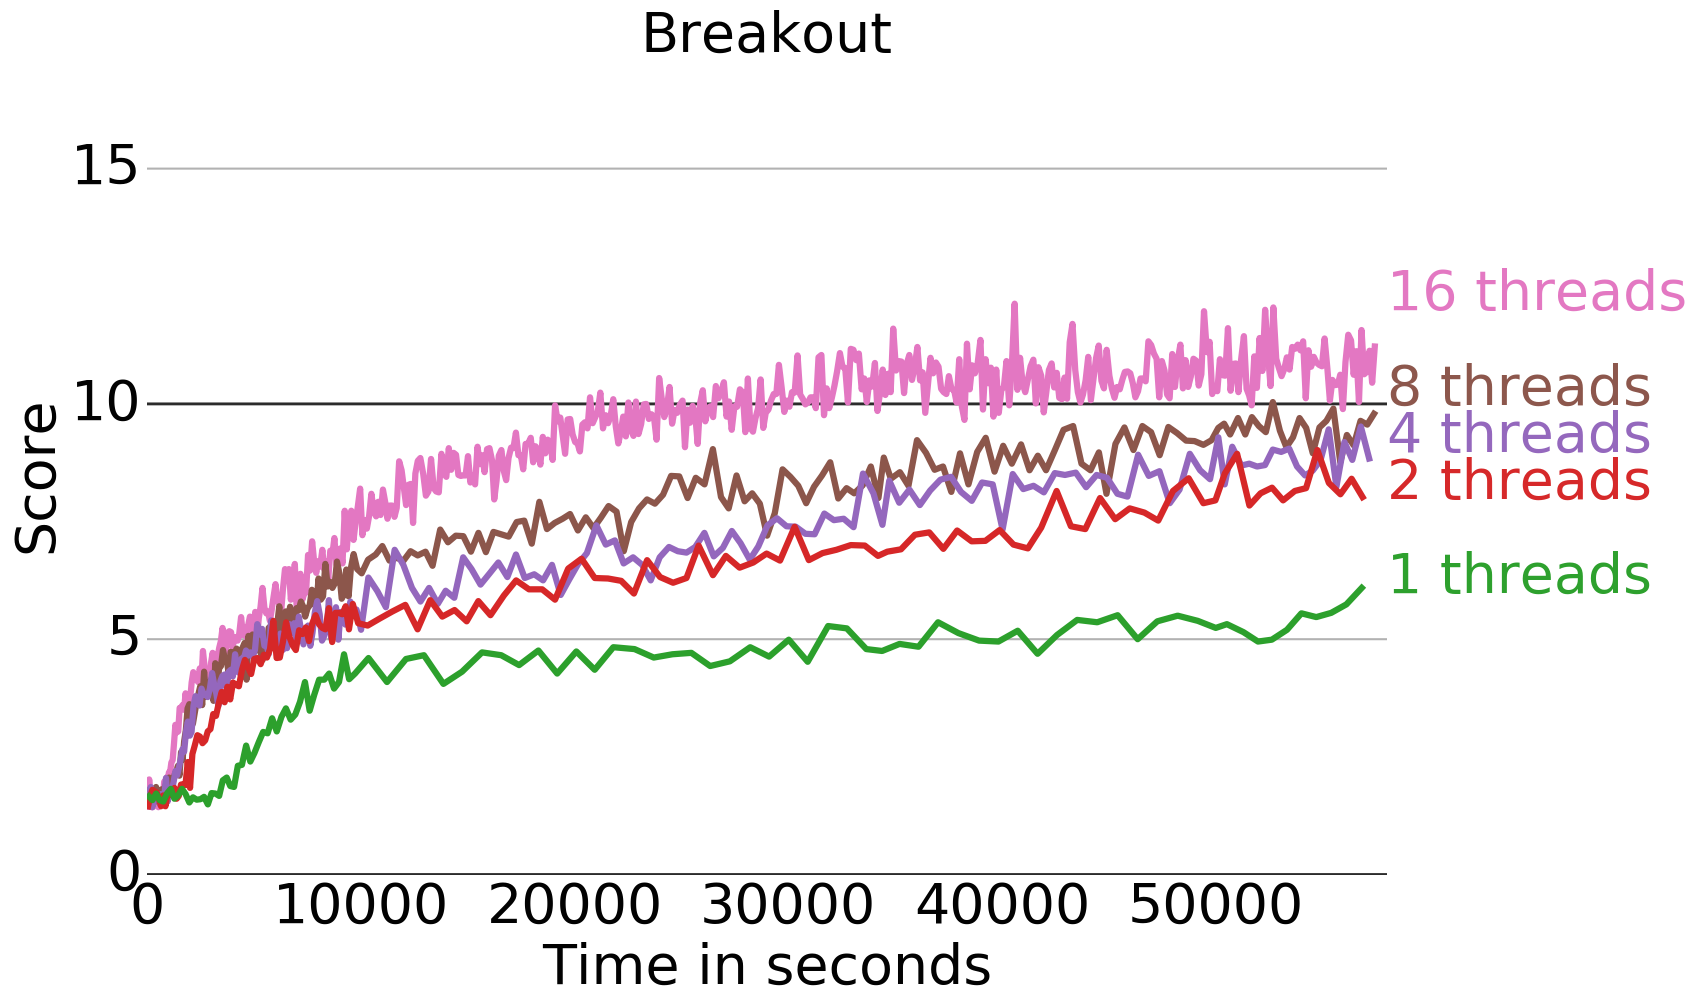
\includegraphics[width=.95\textwidth]{plots/breakout_intro.png}}
        \caption{Score achieved in Breakout as a function of
        consumed real-time.}
    \end{subfigure}
    \begin{subfigure}[t]{.32\textwidth}
        \fbox{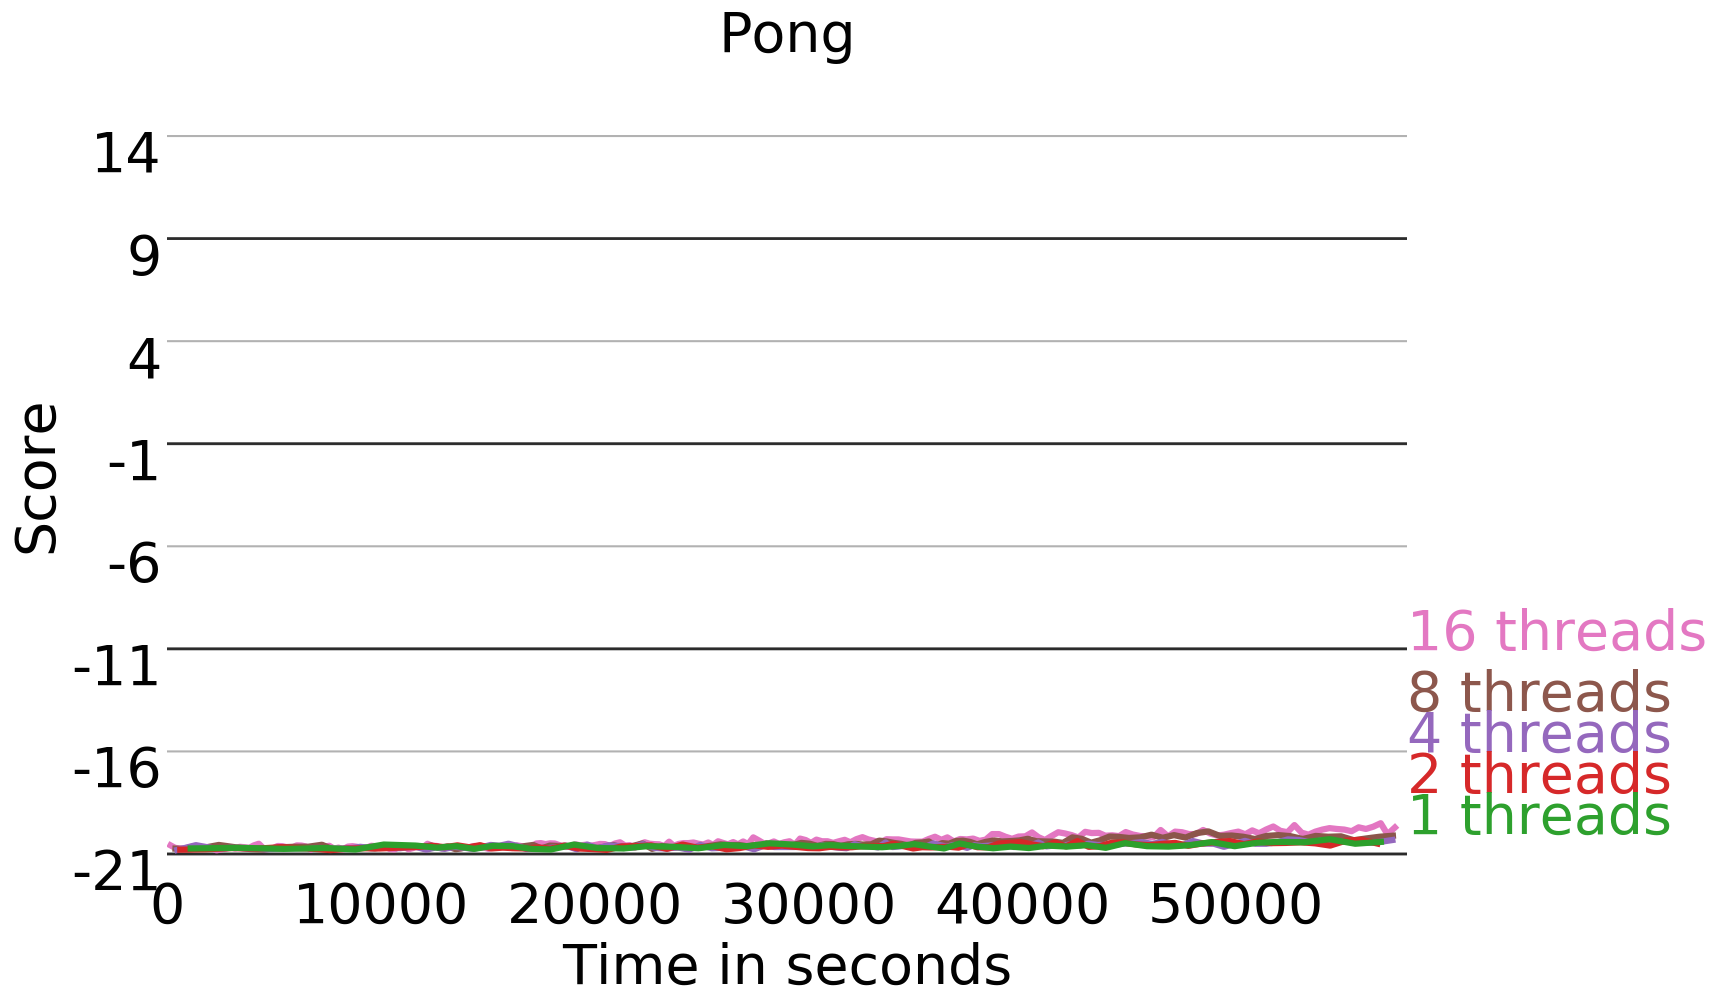
\includegraphics[width=.99\textwidth]{plots/pong_intro.png}}
        \caption{Score achieved in Pong as a function of
        consumed real-time.}
    \end{subfigure}
  \end{tabular}
  \label{fig:all_atari}
  \caption{Results for the three games we have tested our implementation
           of A3C on.}
\end{figure}

From these results it seems as if the implementation is able to learn
a decent policy for both Space Invaders and Breakout, but fails
to learn how to play Pong.

Upon further inspection of Space Invaders, it seems as if
a higher amount of threads leads to a higher score, which is unsuspected
compared to the results from the CartPole problem.
In figure \ref{fig:a3c_spaceinvaders} a view of the results from
playing Space Invaders with all the different thread settings.
Here the plot has been smoothed such that each point represents the mean of the
50 surrounding points.

\begin{figure}[H]
    \fbox{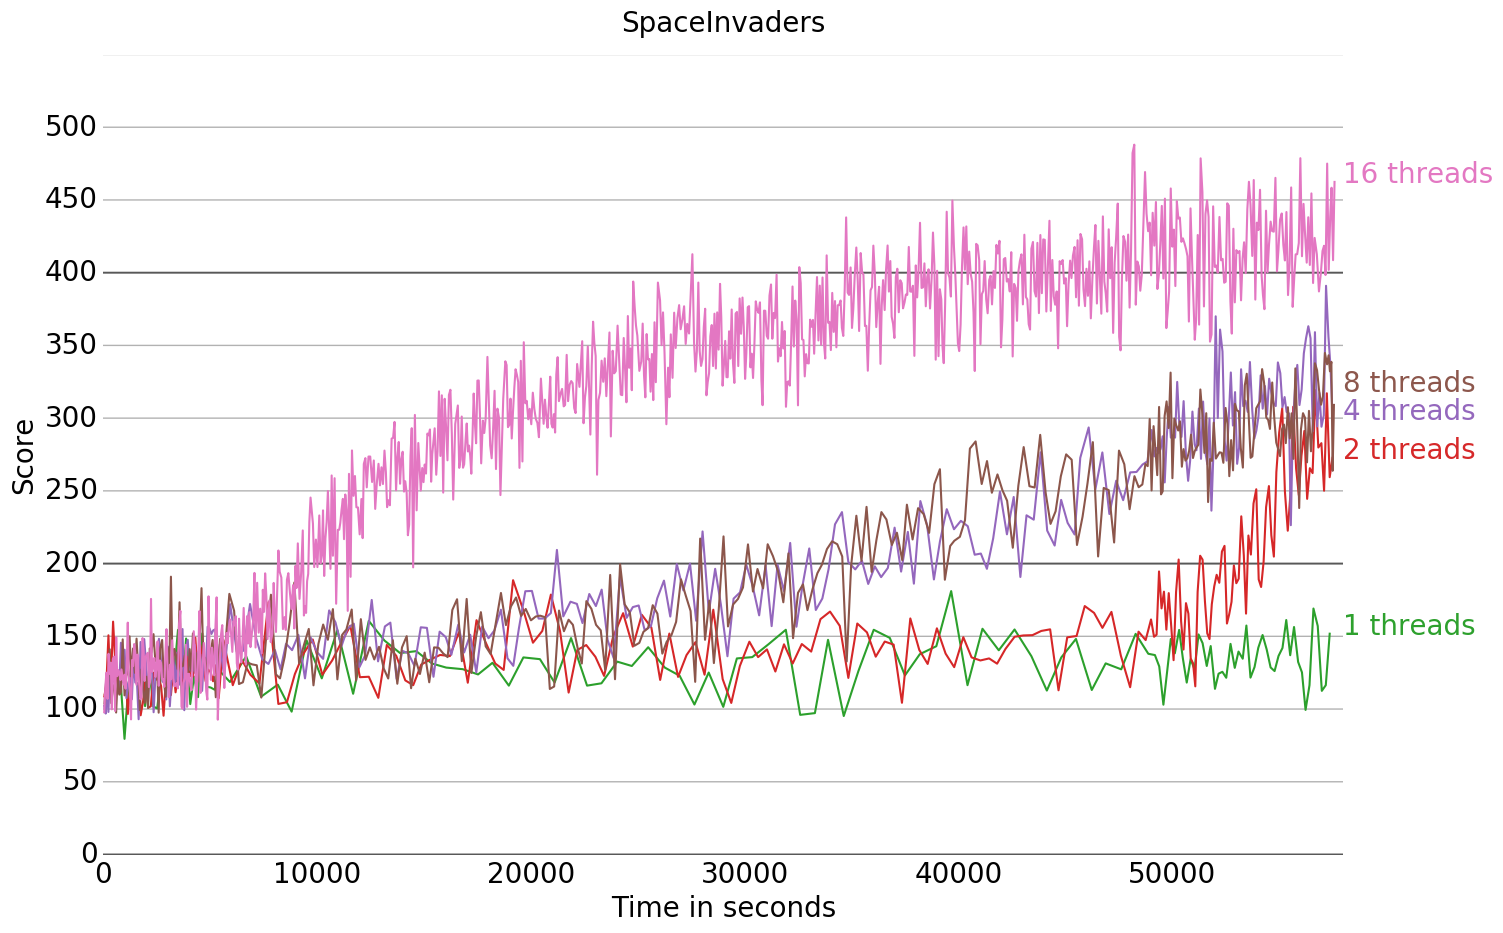
\includegraphics[width=.95\textwidth]{plots/spaceinvaders_compare_score_time.png}}
    \caption{Score achieved in Space Invaders as a function of
    consumed real-time.}
    \label{fig:a3c_spaceinvader}
\end{figure}

Figure \ref{fig:a3c_spaceinvaders_ts} shows the same plot, with the
exception that the score is a function of the timesteps taken
during the experiment.

\begin{figure}[H]
    \fbox{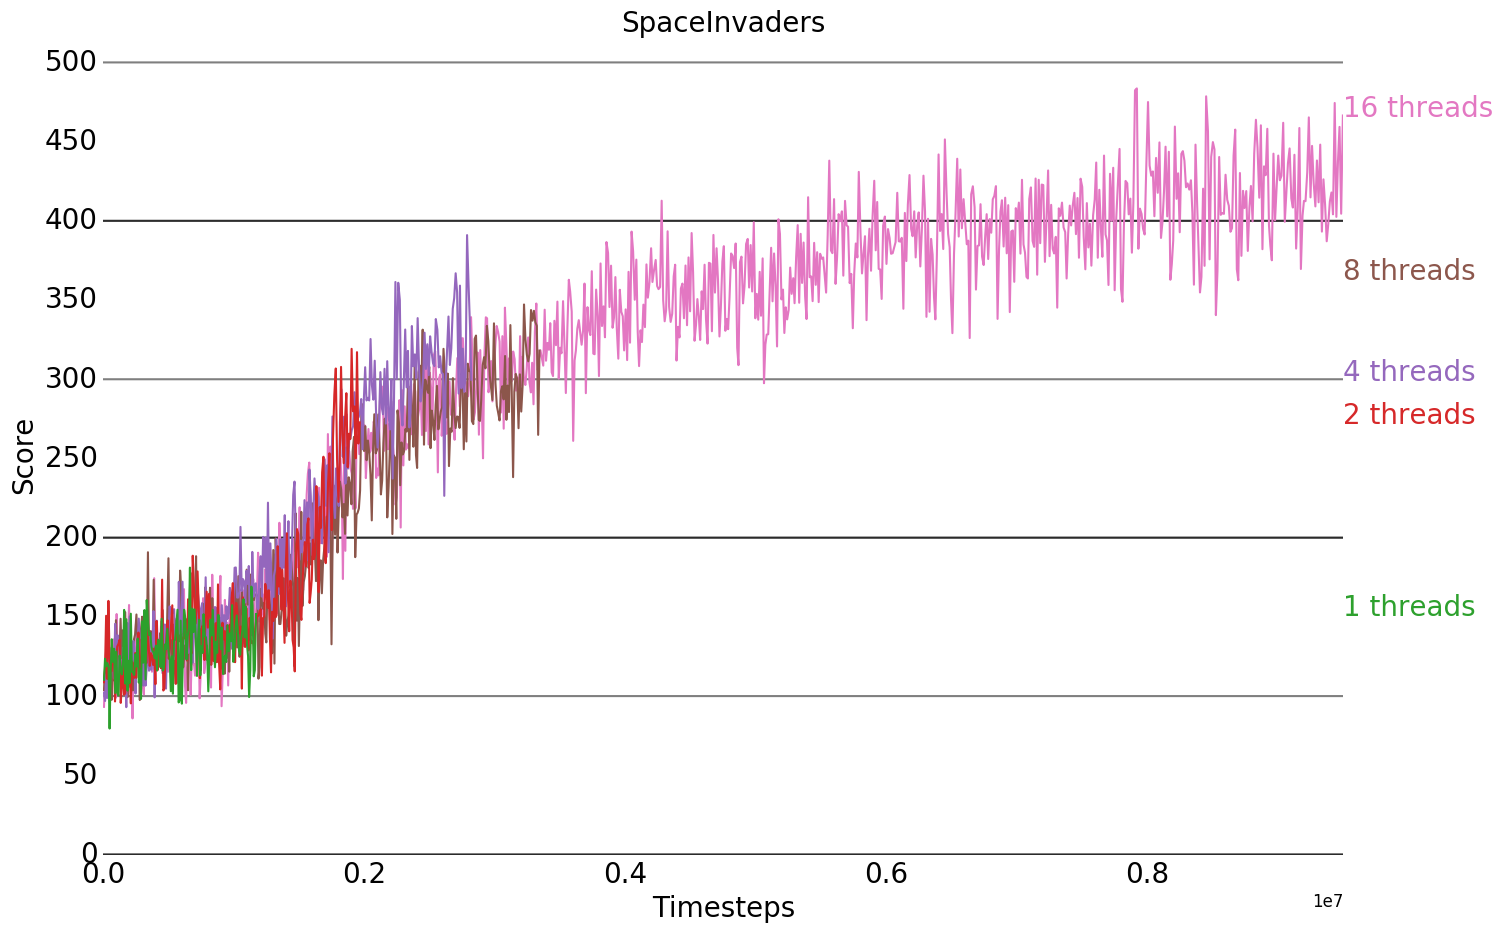
\includegraphics[width=.95\textwidth]{plots/spaceinvaders_score_timesteps.png}}
    \caption{Score achieved in Space Invaders as a function of
    timesteps taken.}
    \label{fig:a3c_spaceinvaders_ts}
\end{figure}

Examining this plot shows that the result of the A3C implementation
on Space Invaders behaves the same way as A3C on CartPole if the threads
were allowed to run for the same amount of timesteps.
The same trend can be seen for Breakout, which is shown in figure
\ref{fig:a3c_breakout_comp}.

\begin{figure}[H]
  \centering   
  \begin{tabular}[c]{cc}
    \begin{subfigure}[c]{.5\textwidth}
        \fbox{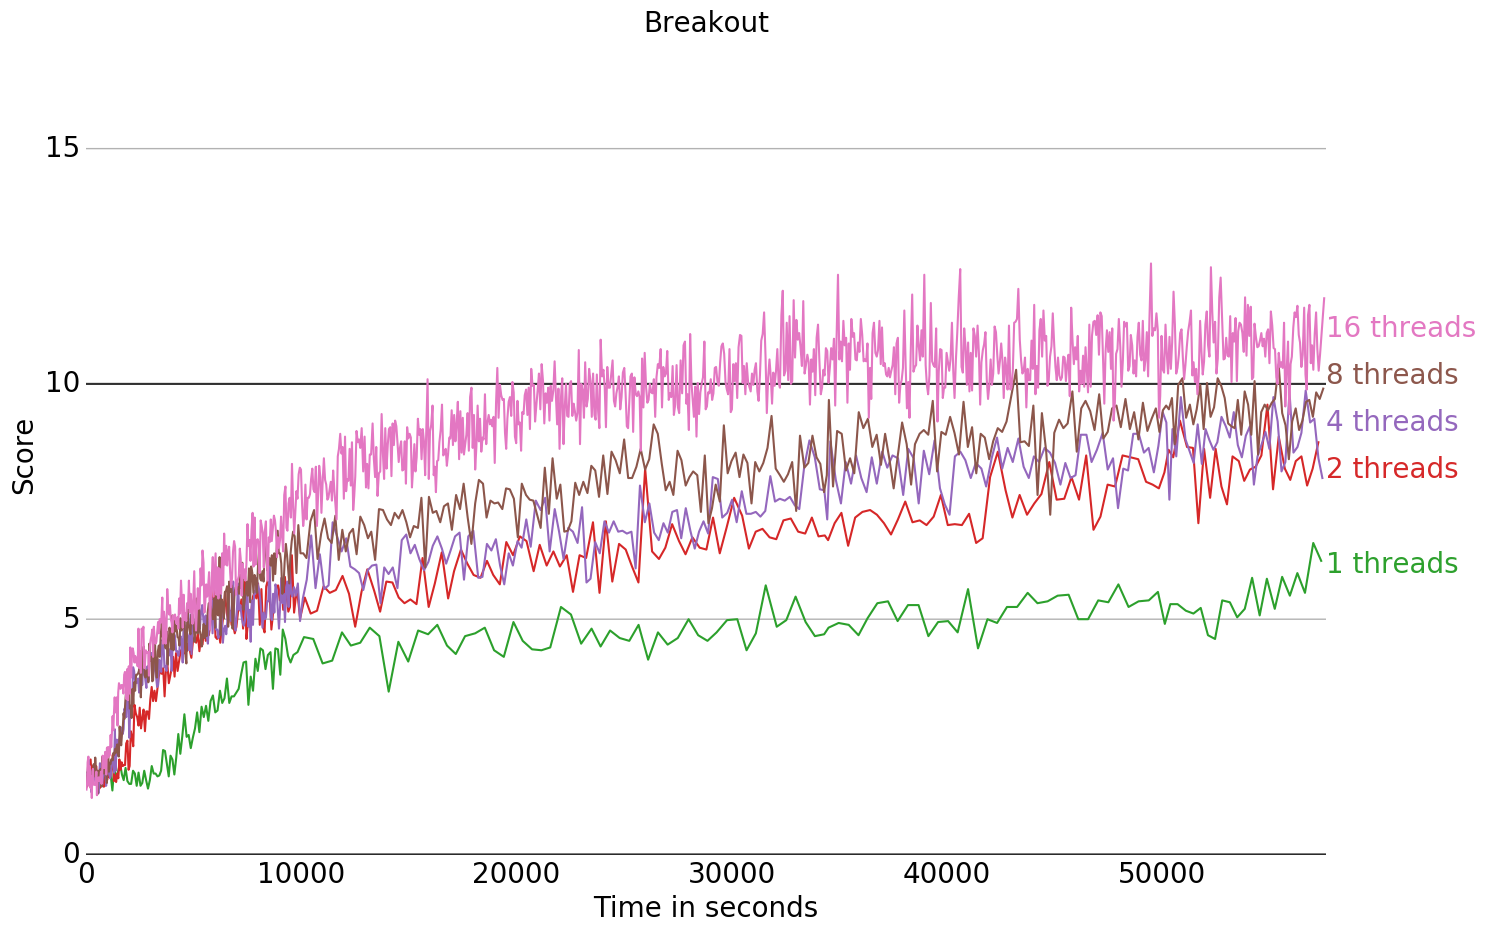
\includegraphics[width=0.97\textwidth]{plots/breakout_compare_time.png}}

        \caption{Score achieved in Breakout as a function of consumed real-time.}
    \end{subfigure}
    \begin{subfigure}[c]{.5\textwidth}

        \fbox{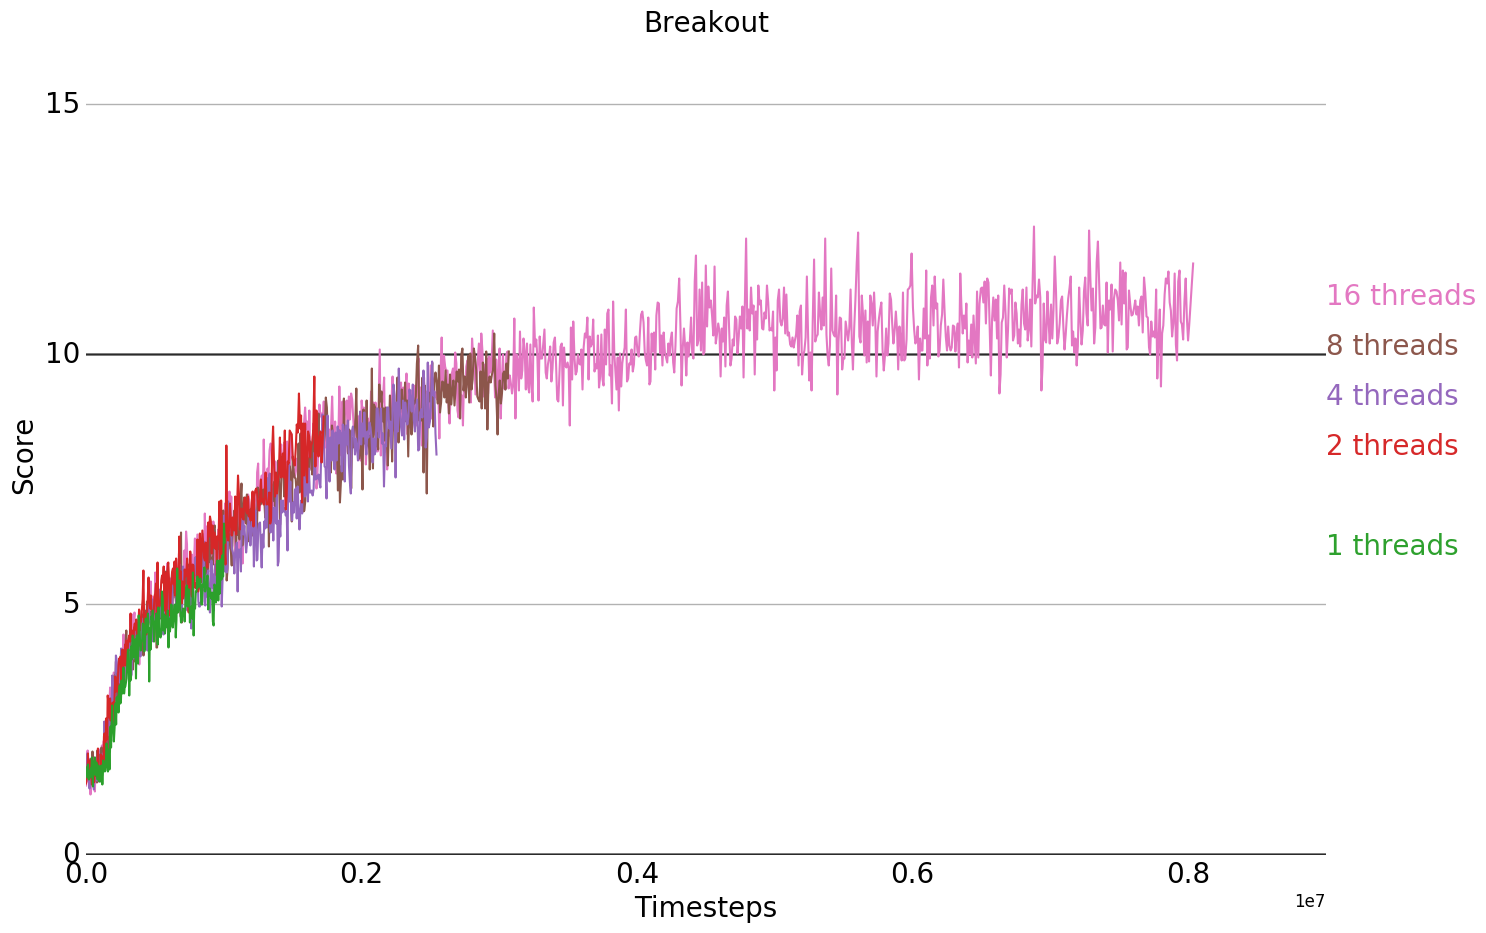
\includegraphics[width=0.97\textwidth]{plots/breakout_steps.png}}
        \caption{Score achieved in Breakout as a function of 
        timesteps taken.}
    \end{subfigure}
  \end{tabular}
  \caption{The scores of all the different thread settings for the
    A3C implementation playing CartPole as a function of timesteps taken.}
     \label{fig:a3c_breakout_comp}
\end{figure}

We have also tested our A3C implementation on the pong enviroment, the
training time have been the same as in Breakout and Spaceinvaders, but
as seen below we got some significant different results.

\begin{figure}[H]
  \centering   
  \begin{tabular}[c]{cc}
    \begin{subfigure}[c]{.5\textwidth}
        \fbox{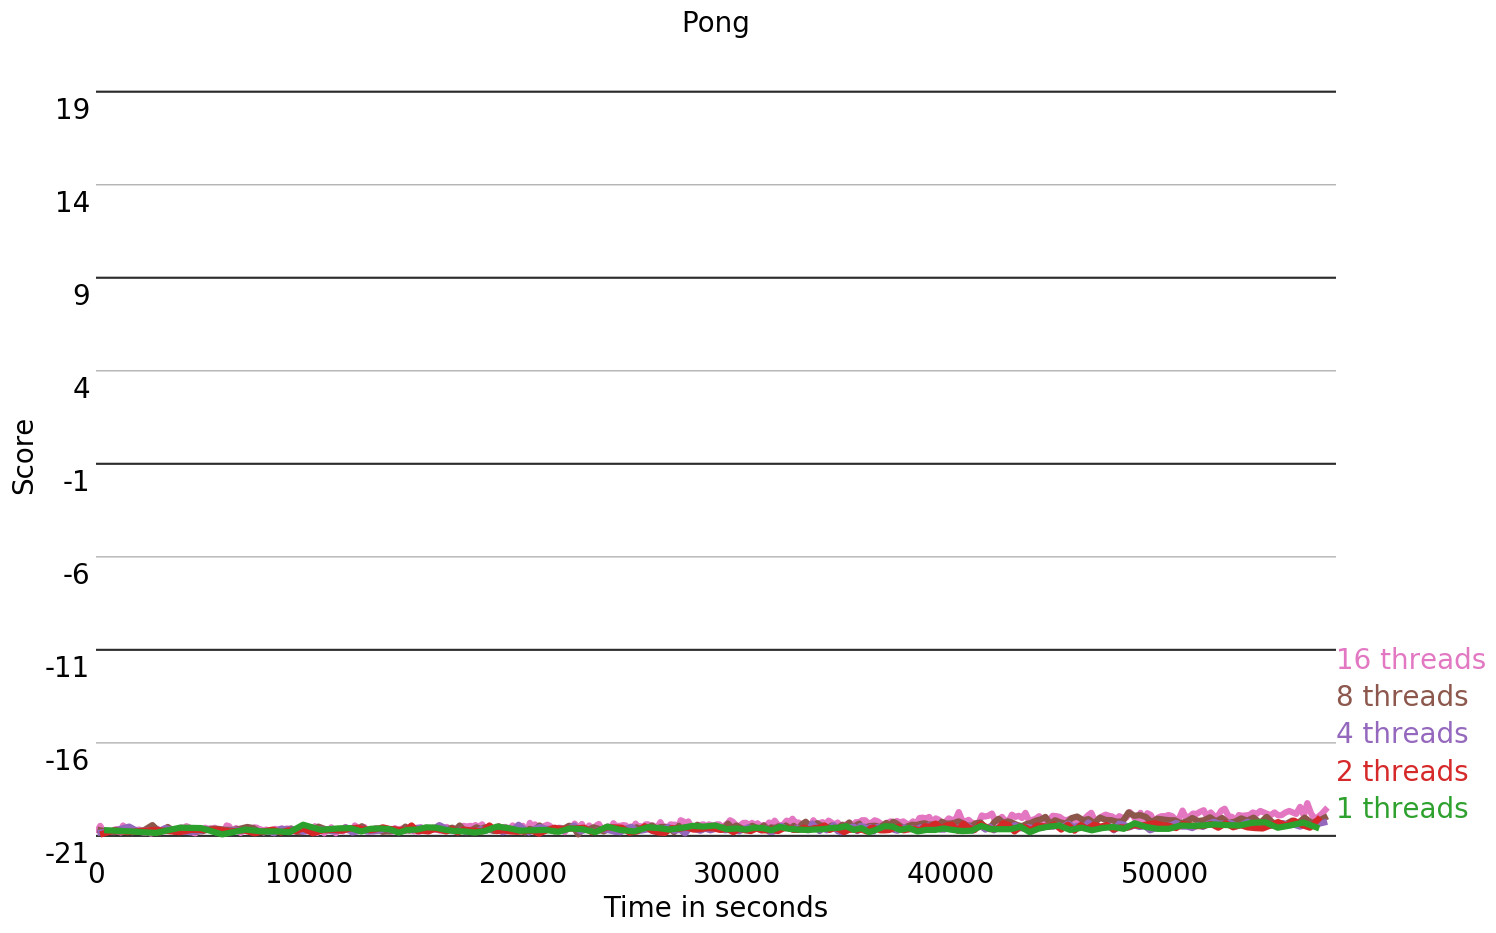
\includegraphics[width=0.97\textwidth]{plots/pong_time.png}}

        \caption{Score achieved in Pong as a function of consumed real-time.}
    \end{subfigure}
    \begin{subfigure}[c]{.5\textwidth}

        \fbox{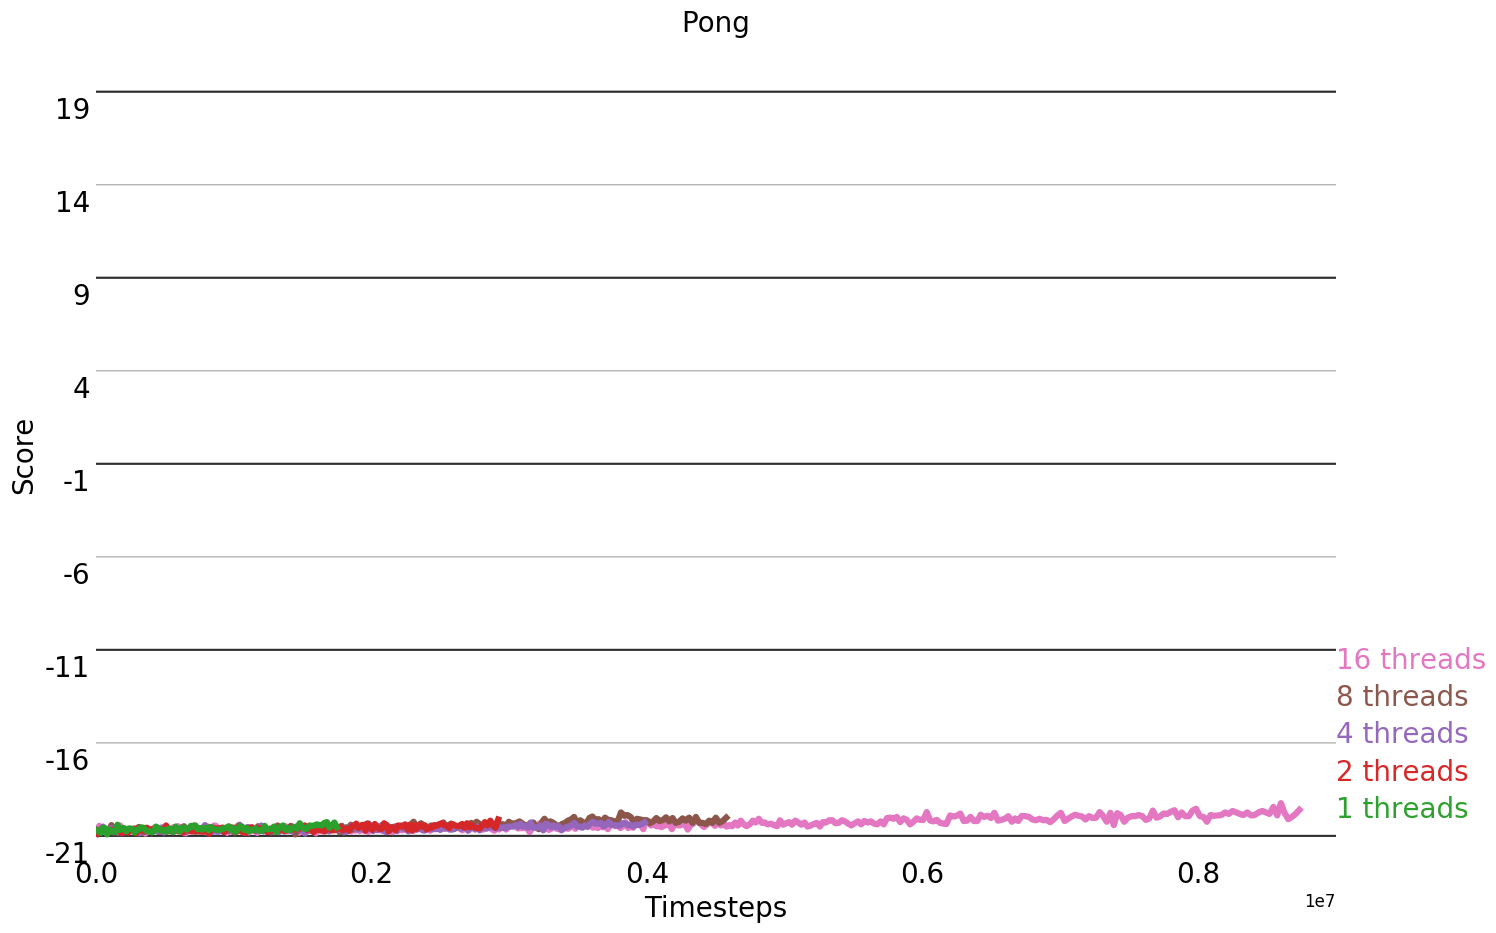
\includegraphics[width=0.97\textwidth]{plots/pong_steps.png}}
        \caption{Score achieved in Pong as a function of 
        timesteps taken.}
    \end{subfigure}
  \end{tabular}
  \caption{The scores of all the different thread settings for the
    A3C implementation playing CartPole as a function of timesteps taken.}
     \label{fig:a3c_pong_comp}
\end{figure}

At the results from figure \ref{a3c_pong_comp}, we general see no improving on
the performance for playing Poing for any of the threads settings. If
we look closely at the results when comparing number of timesteps with
the score, it seems that the 16 threads setting, have a very small
improvment after 900.000 timesteps compared to the start. In section \ref{sec:discussion}
we will discuss why we learn to solve problem, and other don't, and
which difference there are between the games.
\end{document}
